% !TeX root = ../main.tex

\section{Problem Definition}
    \frame{\sectionpage}

    \begin{frame}{Seat Planning with Social Distancing}
      \begin{itemize}
      \item Group type $[M] = \{1, \ldots, M\}$
      \item Row $[N] = \{1, \ldots, N\}$
      \item $s$ seats as the social distancing
      \item Let $n_i = i + s$ denote the new size of group type $i$ for each $i \in [M]$.
      \item Let $L_j = S_j + s$ denote the length of row $j$ for each $j \in [N]$, where $S_j$ represents the number of seats in row $j$.
      \end{itemize}
      
      \begin{figure}[ht]
        \centering
        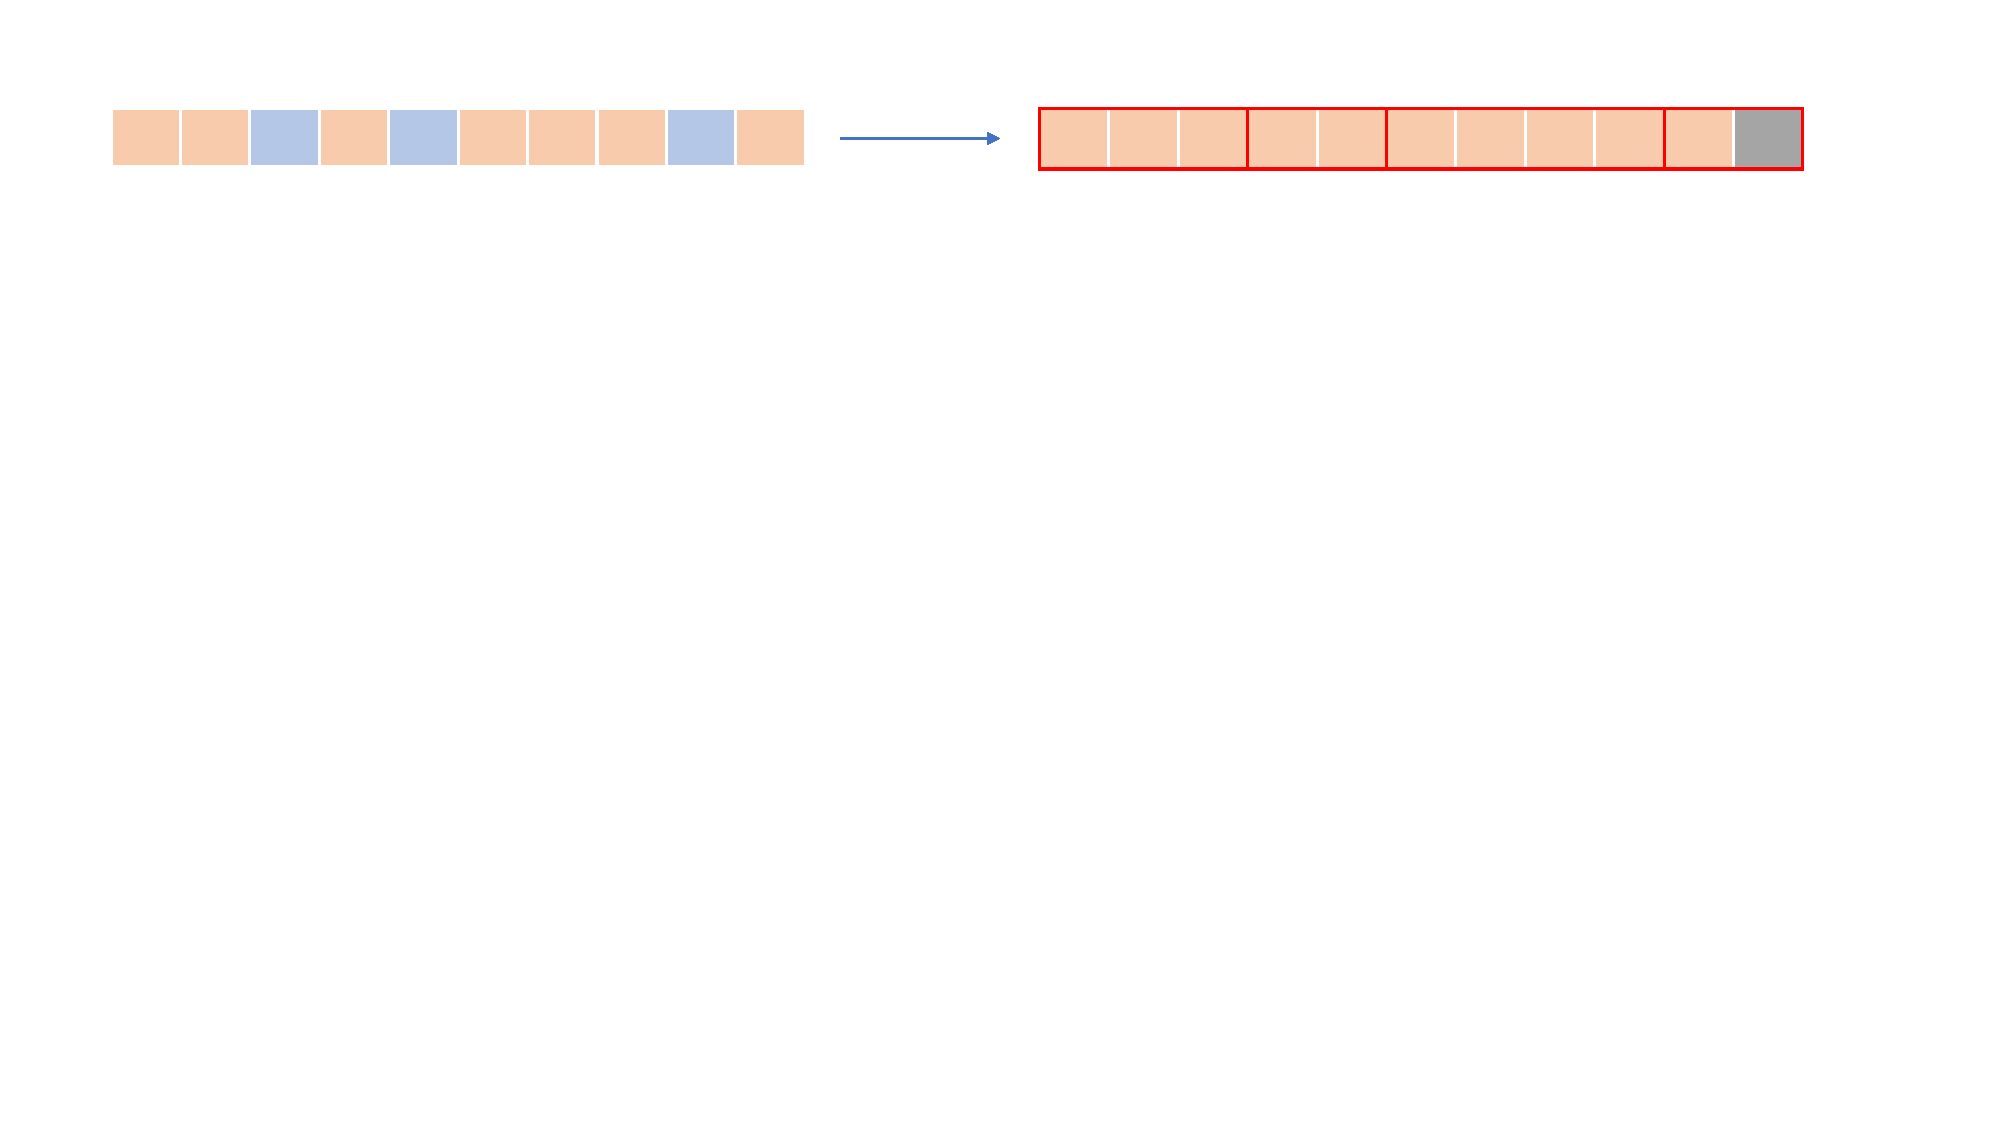
\includegraphics[width = 0.8\textwidth]{./images/dummy_seat.pdf}
        \caption{Problem Conversion}
    \end{figure}
    \end{frame}

    \begin{frame}{Dynamic Programming}
      \centering
      Dynamic seat assignment can be characterized by DP:
      $$V_{t}(\mathbf{L}) = E_{i} \left[ \max_{k \in N: L_k \geq i + s} \{ {[V_{t-1}(\mathbf{L}- U_{ik})+ i]}, {V_{t-1}(\mathbf{L})}\} \right], \mathbf{L} \geq \mathbf{0}$$
      $$V_{T+1}(\mathbf{L}) = 0,$$

      \begin{itemize}
        \item $\mathbf{L} = \{  \}$, remaining capacity.
        \vspace{10pt}
        \item $U_{ik}$
        \vspace{10pt}
        \item $p_i$: the probability of an arrival of group type $i$.
      \end{itemize}
  \end{frame}


  \begin{frame}{Example}
    Suppose the social distancing is one seat, then the new sizes of groups are $2, 3, 4, 5$, respectively. 
    
    The length of one row is $L = 21$.
    
    The demand is $[10, 12, 9, 8]_d$. Then these patterns, $(5, 5, 5, 5, 1), (5, 4, 4, 4, 4),(5, 5, 5, 3, 3)$, belong to $I_1$. 
    
    For pattern 1, $(5, 5, 5, 5, 1)$, $P_{1} = \{5\}$, thus a group with a size smaller than 5 cannot be put in this pattern.
  \end{frame}

  \begin{frame}{Properties}
    \begin{itemize}
      \item $\alpha_k$ indicates the number of items for pattern $k$. $\beta_k$ indicates the left space for maximal pattern $k$. Notice that the left space is the true loss.
      \item Denote $\alpha_k + \beta_k- 1$ as the loss for pattern k, $l(k)$. When $l(k)$ reaches minimum, the corresponding pattern $k$ is the optimal solution for a single row.
      \item If the group sizes are consecutive integers starting from 2, $\{2,3,\ldots,u\}$, then a greedy-based pattern is optimal, i.e., select the maximal group size,$u$, as many as possible and the left space is occupied by the group with the corresponding size. The loss is $k+1$, where $k$ is the number of times $u$ selected. Let $S = u\cdot k + r$.
    \end{itemize}
  \end{frame}

  \begin{frame}{Property}
    \begin{itemize}
      \item Let $I_1$ be the set of patterns with the minimal loss.
      \item 
      \item For a seat layout, $\{S_1, S_2, \ldots, S_{N}\}$, the total loss is $\sum_{j} (\lfloor \frac{S_j+1}{u} \rfloor - f((S_j +1)\mod u))$. The maximal number of people assigned is $\sum_{j} (S_j - \lfloor \frac{S_j+1}{u} \rfloor + f((S_j +1)\mod u))$.
    \end{itemize}
  \end{frame}
  
